\chapter{Obiettivi della tesi}
\label{capitolo3}
\thispagestyle{empty}

L'obiettivo di questa tesi è quello di illustrare le modifiche, le aggiunte ed i cambiamenti effettuati al software di LIS per permettere un integrazione dei ricevitori di allarme in maniera più veloce e standard, una seconda parte della tesi complementare alla prima si focalizza invece sulla telegestione del delle centrali di allarme. 
\section{La situazione iniziale}
Al nostro arrivo in LIS la situazione che si presentava era poco chiara e non ben definita. Gli operatori di centrale che gestivano gli allarmi utilizzavano un software denominato \emph{E-Pro}. Questo programma è un adattamento di un programma utilizzato da \emph{Cobra S.p.a} per la gestione degli allarmi provenienti da veicoli ed è stato adattato  negli anni alla gestione degli impianti fissi.\\
Questo software è un formato da un insieme di moduli alcuni scritti in C ed altri in Java, la parte che riguarda la ricezione degli allarmi il loro immagazzinamento nel database e la logica che gestisce il comportamento da intraprendere per la loro gestione è implementato in una serie di moduli scritti in C; questi moduli sono chiamati:
\begin{itemize}
	\item cp220\_4
	\item cp220\_3
	\item MTSfe\_fissi
\end{itemize}
Questi tre moduli si occupano della ricezione degli allarmi dai vettori PSTN e GPRS/GSM per fare questo utilizzano dei ricevitori fisici chiamati
\begin{description}
	\item[System III:] si occupa della ricezione degli allarmi sul vettore PSTN tramite protocollo Contact ID.
	\item[OHLan:] questo ricevitore è un PC fisico collegato nella rete locale sul quale è installato un software della UTC Fire \& Security che si occupa della ricezione tramite protocollo proprietario degli allarmi provenienti dalle centrali UTC.
	\item[Modem GSM:] più di un modem GSM è collegato ad una porta multi seriale connessa nella rete locale questi modem permettono la ricezione degli allarmi tramite vettore GSM e GPRS per quelle periferiche di backup di derivazione automotive.
\end{description}
Per quanto riguarda la parte Java essa si occupa dell'interazione con l'operatore e quindi il compito di questi moduli è quello di prelevare gli allarmi dal database e mostrarli all'operatore, inoltre,essi si occupano, anche, di tenere traccia di tutte le azioni eseguite dall'operatore. Questa parte è strutturata in modo da garantire la multiutenza, infatti, questi moduli sono scritti in Java EE e sono eseguiti su di un server JBoss in modo da permettere l'esecuzione di più sessioni contemporaneamente.
\begin{figure}
\centering
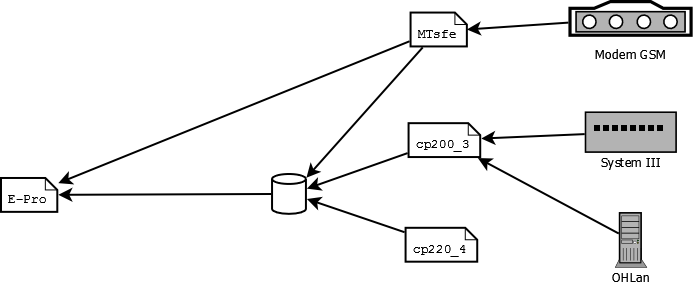
\includegraphics[width=0.9\linewidth]{pictures/struttura.png}
\caption{Schema dei moduli applicativi di LIS}\label{img:struttura}
\end{figure}
\subsection{cp220\_4}
Il \emph{cp220\_4} ha la funzione di leggere e trasformare gli allarmi provenienti dai sistemi di ricezione come il \emph{System III} o lo \emph{OHLan} e di immagazzinarli in un database non prima di averli trasformati in un formato interpretabile dall'E-Pro. Questo formato è derivato direttamente dal Contact ID il prevedere diversi campi
\begin{center}
	\texttt{ACCT MT QXYZ GG CCC S}
\end{center}
dove le diverse sigle indicano:
\begin{description}
	\item[ACCT:] è un identificativo assegnato al cliente
	\item[MT:] è un numero che indica il tipo di messaggio, se esso è nuovo oppure una ritrasmissione.
	\item[XYZ:] è un codice che indica il tipo di evento che è avvenuto
	\item[Q:] un numero che può essere 1 o 3 ed indica se l'evento trasmesso è rispettivamente iniziato o finito.
	\item[GG:] è il numero che identifica la partizione nella quale è stato generato l'allarme
	\item[CCC:] è un numero che identifica il sensore o zona che ha generato l'allarme.
	\item[S:] valore di checksum per il controllo degli errori
\end{description}
Il \texttt{cp220\_4} utilizza i campi ACCT, XYZ, Q, GG, CCC insieme al all'orario nel quale arriva il messaggio e li inserisce in una tabella del database dal quale poi saranno prelevati ed inviati all'operatore.\\
Oltre a questa funzione il modulo all'arrivo di ogni messaggio aggiorna un campo in una tabella chiamata \texttt{seriale} utilizzata controllare periodicamente lo stato in vita dei ricevitori e la loro connessione con il modulo in questione.\\
Questo modulo è il più interessante per noi in quanto è quello che permette la ricezione degli allarmi e quindi il modulo sul quale ci concentreremo per sviluppare la nostra applicazione di ricezione; in realtà esso ci servirà per comprendere la logica che un ricevitore deve eseguire una volta ricevuto l'allarme.
\subsection{cp220\_3}
Questo modulo si occupa della logica della gestione degli allarmi per capire meglio il funzionamento di questo modulo facciamo un esempio e consideriamo un locale commerciale con prefissati orari di apertura e di chiusura. Il sistema di allarme viene disinserito poco prima dell'apertura, in questo caso alla centrale arriva l'evento di disinserimento dell'impianto ma il cp220\_3 controlla l'orario di arrivo di tale evento e calcola che questa segnalazione è conforme all'orario di apertura e quindi lo registra ma non lo inoltra agli operatori di centrale. Nel caso in cui, invece, tale evento di disinserimento si verifica durante le ore notturne, e quindi fuori dal normale orario di apertura allora il software verifica l'anomalia e invia la segnalazione all'operatore che provvederà a gestirla.\\
Il \texttt{cp220\_3} si occupa di capire quali segnalazioni inviare all'operatore. Oltre al controllo orario visto in precedenza, si occupa di filtrare le segnalazioni multiple provenienti ad esempio da ritrasmissioni, di filtrare gli impianti in test o disattivati che comunque inviano segnalazioni alla centrale.
\subsection{MTSfe}
Lo \texttt{MTSfe} è un software che deriva da \emph{Cobra Italia} e si occupa principalmente della gestione delle periferiche di backup di derivazione automotive ovvero delle periferiche \emph{PowerSat}. Queste periferiche erano state pensate per il controllo di autoveicoli e sono state adattate all'utilizzo negli impianti fissi come periferiche di backup in quanto sono dotate di una decina di ingressi programmabili e di alcune contatti di uscita.\\
Questo modulo pur essendo rimasto parte integrante del software di LIS è ancora di proprietà di Cobra Italia è perciò stato impossibile per noi modificarlo, tuttavia uno dei nostri obiettivi a lungo termine era quello di sostituire le vecchie periferiche di backup PowerSat con altre più preformanti e aperte così da poter essere gestite direttamente dal nuovo software.
\subsection{E-Pro}
\emph{E-Pro} è il software centrale che gestisce l'interazione tra operatore e sistema. Mentre i moduli in C si occupano di ricevere e selezionare gli allarmi il software E-Pro si preoccupa di prelevarli dal database e mostrarli all'operatore per poi aiutarlo nella gestione e controllo della segnalazione.\\
Questo software è composto da una serie di moduli Java EE che vengono eseguiti in un ambiente JBoss. Questi moduli hanno compiti diversi e svolgono le diverse funzionalità tra cui:
\begin{itemize}
	\item autenticazione e profilazione degli utenti che utilizzano E-Pro;
	\item gestione dell'interfaccia grafica;
	\item elaborazione finale degli allarmi;
	\item gestione della reportistica.
\end{itemize}
\section{Obiettivi della tesi}
Gli obiettivi di questa tesi sono diversi e intervengono su diversi aspetti del software preesistente ma tutti questi obiettivi si prefiggono lo scopo principale di strutturare il software in maniera adeguata per permettere l'estensione delle funzionalità in modo rapido e strutturato permettendo così in futuro di non dover ripensare e riscrivere il software per integrare nuovi protocolli o aggiungere nuove funzionalità al software.
\subsection{Integrazione di nuovi protocolli in minor tempo}
Il primo degli obiettivi che vogliamo analizzare è quello dell'integrazione dei nuovi protocolli. Per prima cosa dobbiamo fare una piccola distinzione in due casi il primo caso si ha quando le segnalazioni di allarme arrivano da un ricevitore esterno come avveniva in precedenza con il System III  in questo caso il protocollo da integrare è quello del ricevitore che si interpone tra la centrale di allarme ed il software di ricezione. Il secondo caso si ha quando la centrale d'allarme comunica direttamente con il software di ricezione.  I due casi se pur distinti sono simili in quanto si può trattare il ricevitore esterno come una centrale d'allarme che comunica gli eventi con identificativi diversi.\\
Per fare ciò si è pensato di sostituire o comunque affiancare al cp200\_4 un nuovo modulo che memorizza gli allarmi sulla base di dati nello stesso modo del cp200\_4 per mantenere la retro compatibilità del software. Questa soluzione è stata una scelta obbligata per non dover riscrivere interamente il software tuttavia, come vedremo nella sezione successiva, non è stata una scelta ottimale.
\subsection{Strutturazione del software}
Il secondo obiettivo che ci siamo prefissati è stato quello di dare al software una struttura più solida e modulare in modo da non dover riprogettare il software in futuro con la richiesta di nuove funzionalità come è stato necessario nel nostro caso. Per fare ciò si è deciso di strutturare anche la parte C in un software ad oggetti con conseguente passaggio obbligato al linguaggio C++. La scelta del linguaggio C++ rispetto al Java è stata una scelta puramente pratica in quanto le nostre conoscenze erano più sbilanciate verso questo linguaggio inoltre, la gestione delle periferiche seriali è più semplice utilizzando tale linguaggio.
\subsection{Telegestione}
Una funzione completamente nuova richiesta dalla centrale operativa era quella di poter telegestire le diverse centrali direttamente dal software E-Pro. Per fare ciò è stato necessario innanzitutto capire quali erano le funzioni necessarie per una corretta telegestione da parte dell'operatore. In secondo luogo è stato necessario capire quali centrali fossero in grado di permettere tali funzionalità e su quale vettore di comunicazione erano disponibili. Infine a livello pratico è stato necessario capire in quale modo implementare tali funzioni.\\
Obiettivi secondari alla telegestione sono stati la minimizzazione dei tempi di reazione del software e lo studio di una nuova interfaccia grafica per esprimere in modo immediato le nuove informazioni messe a disposizione dell'operatore.
\subsection{Utilizzo di nuovi vettori di comunicazione}
Gli obiettivi di rinnovamento del software non potevano limitarsi solamente ad un nuovo software ma, soprattutto, erano legati in modo indissolubile dall'utilizzo di nuovi vettori di comunicazione in particolare TCP/IP, GPRS ed SMS per minimizzare i costi di comunicazione e diminuire i tempi di dialogo tra la centrale di allarme e la centrale operativa.\\
L'utilizzo di questi vettori ha comportato lo studio di protocolli specifici come il Contact-ID o il SIA over IP e l'utilizzo e quindi l'interfacciamento del software con nuovo hardware come i modem GPRS.
\section{Vincoli di progetto}
Con il nostro arrivo sono state introdotte numerose modifiche al software preesistente tuttavia per mantenere l'operatività e l'usabilità durante tutto lo sviluppo è stato necessario effettuare alcune scelte che permettessero la retro compatibilità e la normale esecuzione del software preesistente. In particolare è stato necessario mantenere il meccanismo nel quale il cp220\_4 memorizzava gli allarmi nel database. Questo memorizzazione consisteva nell'inserimento in tabella di un nuovo record composto da diversi campi tra cui il codice della centrale, il codice di allarme, il numero della partizione, della zona, la data e l'ora in cui è avvenuto l'evento e altre informazioni che saranno mostrate in dettaglio nel \chaptername~\ref{capitolo4}.\\
Questo meccanismo tuttavia porta con se diversi problemi.
Il primo problema che si presenta anche se di facile soluzione si ha quando la segnalazione di allarme non porta con se l'ora della segnalazione, questo problema si risolve impostando l'ora della ricezione come ora in cui è avvenuta la segnalazione, tuttavia questo tipo di informazione è superflua in quanto non viene utilizzata in nessuna altra parte del software.\\
Il secondo problema più complesso consiste nel codice di allarme, esso è simile al Contact ID tuttavia, il Contact ID ha una struttura \texttt{QXYZ} dove Q è uno tra i numeri 1, 3 o 5 che indicano rispettivamente il nuovo evento, il termine di un evento e la continuazione di una segnalazione mentre XYZ è un codice identificativo del tipo di evento. mentre la memorizzazione avviene con un codice che ha la forma \texttt{XYZQ} ovvero con il numero rappresentato dalla lettera \texttt{Q} in coda rispetto al Contact ID standard questo comporta delle elaborazioni aggiuntive prima di memorizzare il dato. Inoltre il codice Contact ID non è completamente univoco ma per alcune segnalazioni su centrali differenti avremmo significati diversi questo, in precedenza era stato risolto con una tabella nel database che associava ad un determinato tipo di centrale le corrispondenti etichette con il significato del codice. Questo meccanismo è rimasto invariato tuttavia esso comporta che ad ogni integrazione è necessario aggiungere centinaia di record a questa tabella per poter permettere la conversione. L'ultimo problema riscontrato riguardo l'adozione di questo tipo di memorizzazione è stato il fatto che non tutte le centrali comunicano tramite protocollo Contact ID e questo ha comportato l'introduzione di una tabella di traduzione per convertire i codici provenienti da altri protocolli in codici Contact ID.\\
Un problema che abbiamo riscontrato sempre riguardante i codici Contact ID riguardava il valore del campo \texttt{Q} in quanto questo campo è utilizzato dal cp220\_3 per effettuare il controllo orario di un impianto i codici 1401 e 3401 indicano rispettivamente l'inserimento ed il disinserimento da parte dell'utente dell'impianto, il cp220\_3 sfrutta questi due codici per verificare che tali eventi avvengano nelle fasce orarie prestabilite. Questo meccanismo funzionava correttamente per le centrali già integrate in quanto esse rispettavano questi codici per indicare gli inserimenti e i disinserimenti, tuttavia, per alcune centrali integrate durante il nostro percorso ci è capitato di trovarne alcune che invertivano i due codici e questo ci ha obbligati ad utilizzare la tabella di traduzione per mantenere un comportamento corretto del software.\\
Il principale problema riscontrato tuttavia nell'utilizzo del codice precedente è stato proprio la comprensione del suddetto codice sorgente mal commentato, con refusi  di vecchie funzioni provenienti da versioni precedenti e soprattutto la mancanza di una struttura logica del programma, basti pensare che il cp220\_3 e il cp220\_4 sono due programmi che svolgono due funzioni completamente distinte ma che in realtà provengono dallo stesso codice sorgente compilato con parametri differenti. Per ovviare a questo problema abbiamo innanzitutto introdotto il codice in un sistema di controllo versione, eliminato oltre diecimila righe di codice inutilizzato e commentato ogni singola funzione tramite un sistema di generazione della documentazione automatica. Questo ci ha permesso di comprendere le funzionalità del software anche se in alcuni casi non è servito a capirne il reale funzionamento o la logica con la quale è stato programmato; questo non ha causato grosse difficoltà ma potrebbe crearne quando si cercherà di sostituire il cp220\_3 con un nuovo modulo meglio strutturato.


